% ---------------------------------------------------------------------
%  07 · Resultados
% ---------------------------------------------------------------------
% macros de los gráficos TikZ (deben definirse fuera de los frames)
\newcommand{\lat}[5]{% fila, longitud, color, etiqueta, valor
  \node[font=\tiny,anchor=east] at (-1.5,{-#1*7-3}) {#4};
  \fill[#3] (0,{-#1*7-5}) rectangle (#2,{-#1*7-1});
  \node[font=\tiny\bfseries,anchor=west] at (#2,{-#1*7-3}) {#5};}
\newcommand{\gbar}[6]{% y, valor, inf, sup, color, rotulo
  \fill[#5] (0,{#1-1.8}) rectangle (#2,{#1+1.8});
  \draw[uistext,line width=0.5pt] (#3,#1) -- (#4,#1)
    (#3,{#1-1}) -- (#3,{#1+1}) (#4,{#1-1}) -- (#4,{#1+1});
  \node[font=\tiny\bfseries,anchor={\ifdim#2pt<0pt east\else west\fi}]
    at ({min(#2,#3)-0.08+(#2>0)*(max(#2,#4)-min(#2,#3)+0.16)},#1) {#6};}

\seccion{Resultados}

% ---------------------------------------------------------------- OE1
\subseccion{¿La caracterización distingue los regímenes?}
% tarjeta de dispositivo: x0, cifra, texto, diseño, % compute, % memory, nota
\newcommand{\dcard}[7]{%
  \fill[uiscard,rounded corners=1mm] (#1,0) rectangle ++(60,64);
  \node[font=\fontsize{30}{32}\selectfont\bfseries,text=uisgreen] at ({#1+30},55) {#2};
  \node[font=\normalsize] at ({#1+30},44) {#3};
  \node[font=\small,text=uisgray] at ({#1+30},36.5) {#4};
  \fill[uisgreen] ({#1+5},16) rectangle ({#1+5+0.5*#5},25);
  \fill[uislime]  ({#1+5+0.5*#5},16) rectangle ({#1+55},25);
  \node[font=\small\bfseries,text=white] at ({#1+5+0.25*#5},20.5) {#5 \%};
  \node[font=\small\bfseries] at ({#1+5+0.5*#5+0.25*#6},20.5) {#6 \%};
  \node[font=\scriptsize,text=uisgray,anchor=west] at ({#1+5},12.5) {compute};
  \node[font=\scriptsize,text=uisgray,anchor=east] at ({#1+55},12.5) {memory};
  \node[font=\scriptsize,text=uisgray] at ({#1+30},5) {#7};}

\begin{frame}{El conjunto de datos cubre ambos regímenes}
  \vspace{-2mm}\centering
  \begin{tikzpicture}[x=1.1mm,y=0.8mm]
    \dcard{0}{42\,458}{intervalos CPU · 30 familias}{tope de 1000 por familia y clase}{50.3}{49.7}{21\,350 compute · 21\,108 memory}
    \dcard{64}{483}{corridas GPU · 16 familias}{19 kernels × 10 niveles de reloj}{35.4}{64.6}{171 compute · 312 memory}
  \end{tikzpicture}
  \notapie{Ambos se ponderan por celda de familia y clase, para que ninguna domine el entrenamiento y el desbalance no sesgue el modelo. CPU: además, tope de 1000 por celda. GPU: sin tope, las 483 corridas completas. Medido en CPU: 1470 corridas y 1.31 M de intervalos elegibles (40.2 \% \textit{compute}).}
\end{frame}

% ---------------------------------------------------------------- OE2 CPU
\subseccion{Clasificador CPU}
\begin{frame}{En CPU, ningún modelo supera 0.73 con familias no vistas}
  \begin{columns}[c]
    \begin{column}{0.6\textwidth}
      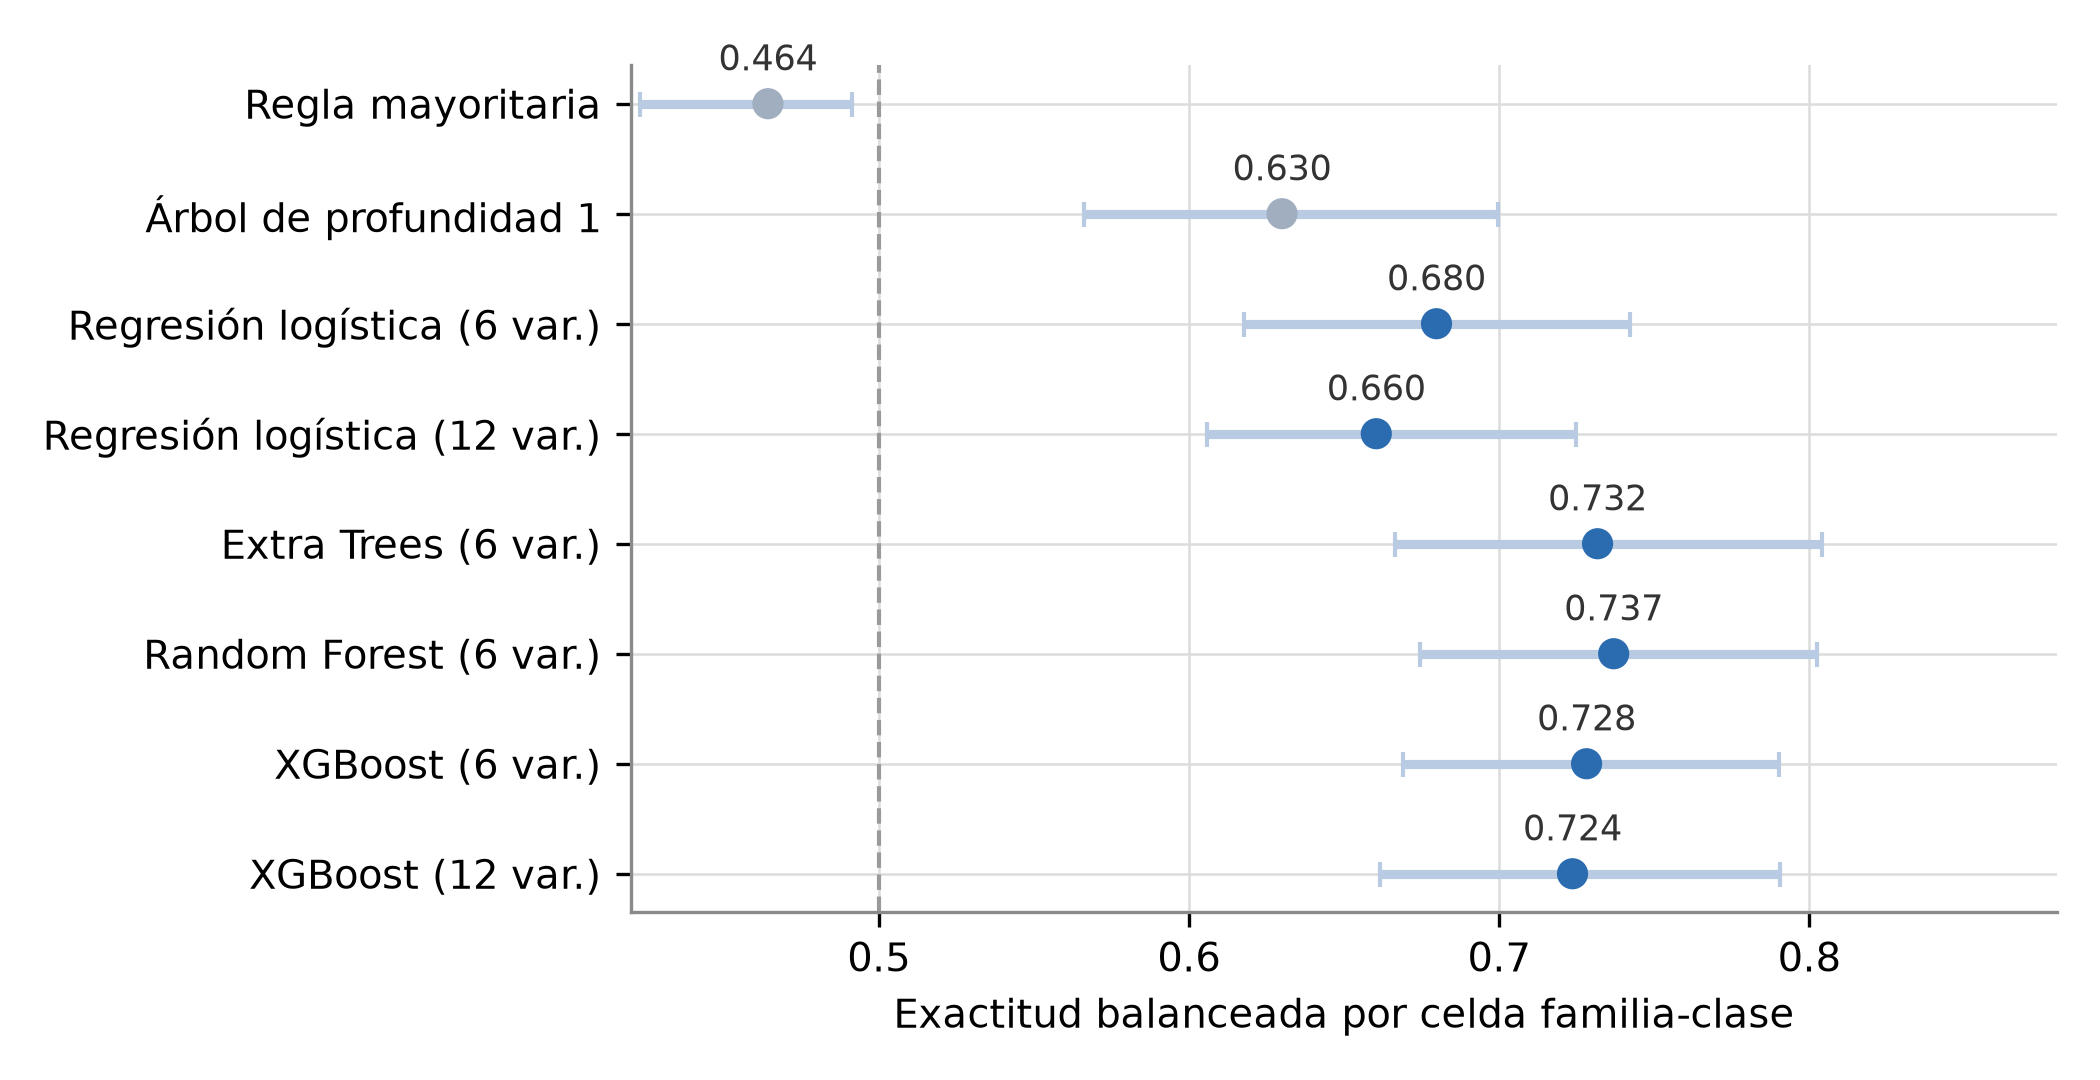
\includegraphics[width=\linewidth]{fig_cpu_comparacion_modelos_20260919.png}
    \end{column}
    \begin{column}{0.38\textwidth}
      \begin{cardhi}[halign=center]
        \bignum{0.728}\\
        XGBoost · exactitud balanceada por celda, familia retirada (IC95 0.669--0.790)
      \end{cardhi}
      \begin{card}
        Los bosques empatan dentro del IC95; XGBoost se eligió por latencia
        (243 µs frente a 5.3 ms en Python)
      \end{card}
      \begin{card}
        Optuna anidado: $+0.019$ (IC95 $-0.007$ a $+0.050$) → configuración fija.
        El límite está en la información, no en el modelo (anexo A5)
      \end{card}
    \end{column}
  \end{columns}
\end{frame}

% ---------------------------------------------------------------- OE2 GPU
\subseccion{Clasificador GPU}
\begin{frame}{En GPU se eligió el modelo que no depende del reloj que el agente modifica}
  \begin{columns}[c]
    \begin{column}{0.56\textwidth}
      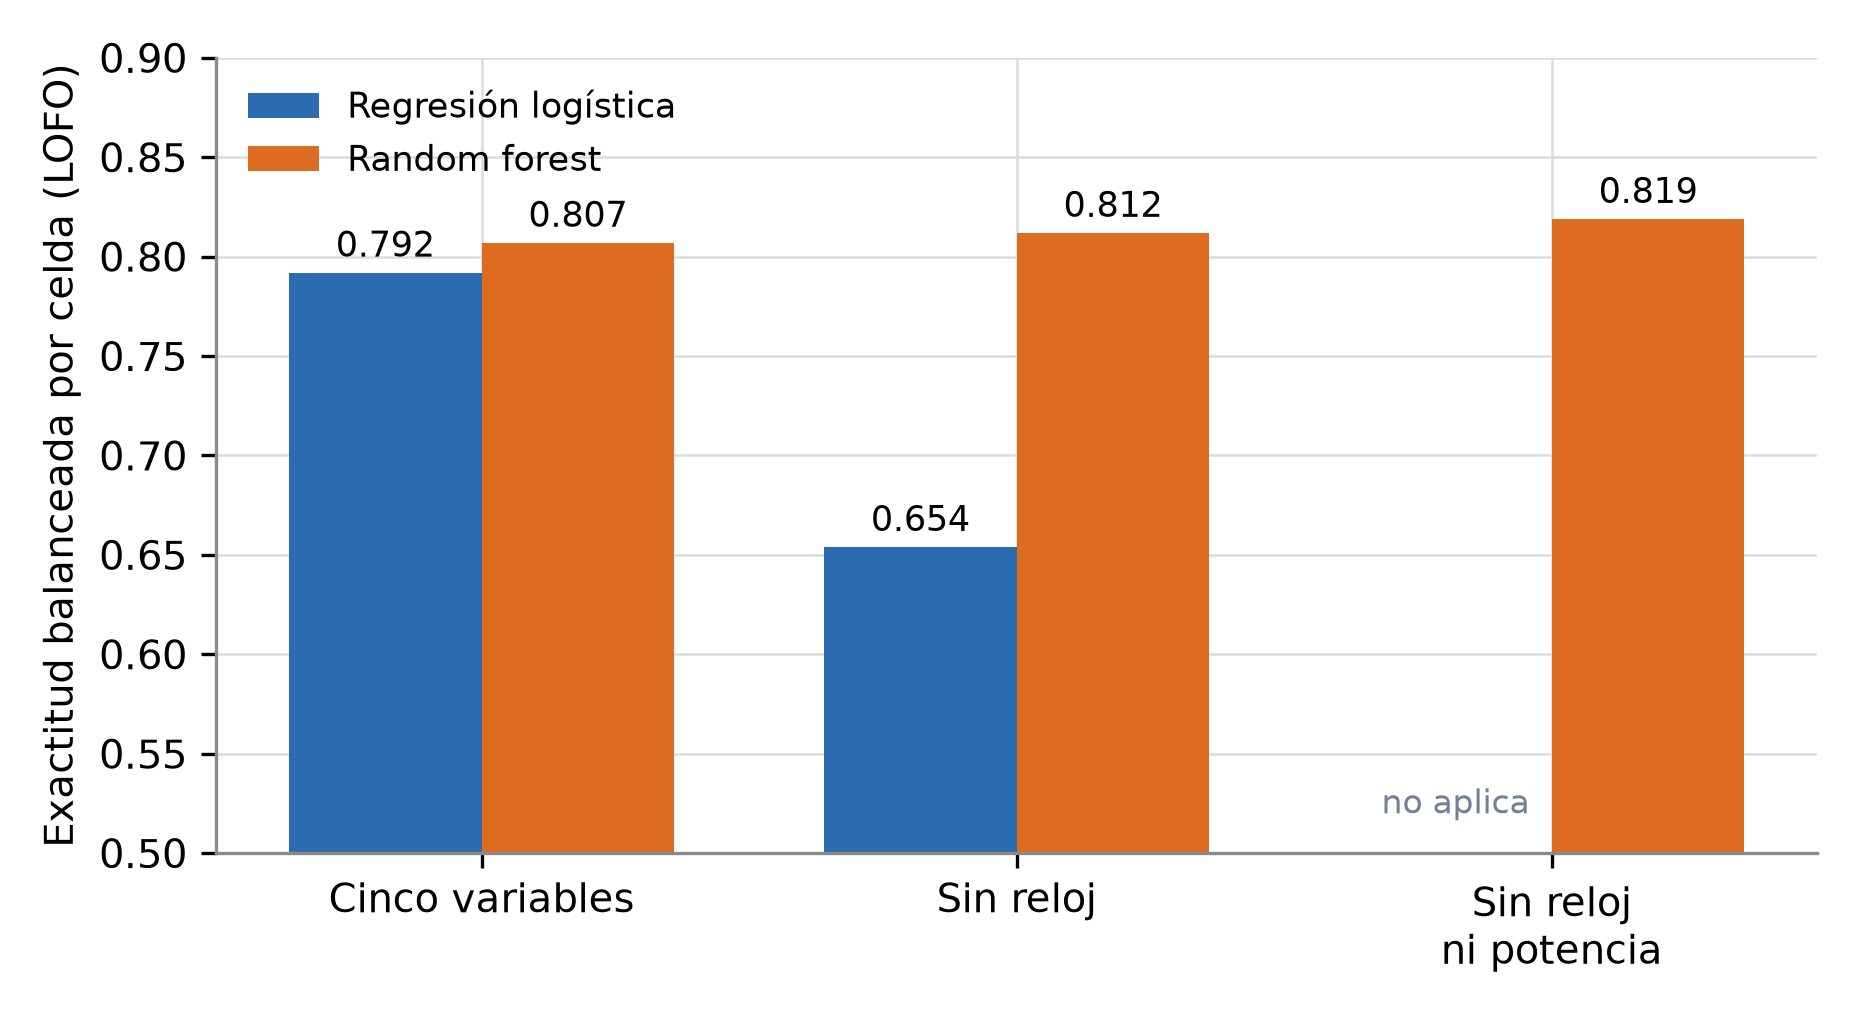
\includegraphics[width=\linewidth]{fig_gpu_invarianza_reloj_20260923.png}
    \end{column}
    \begin{column}{0.42\textwidth}
      \begin{cardhi}[halign=center]
        \bignum{0.819}\\
        \textit{Random forest} con 3 señales invariantes al reloj, familia retirada
      \end{cardhi}
      \begin{card}
        Fijar el reloj en 1410 MHz cambia el 26.7 \% de las predicciones de la
        regresión logística; el RF conserva su exactitud sin reloj ni potencia
      \end{card}
      \begin{card}
        Con $\tau=0.90$: 0.900 de exactitud y cobertura de 65.7 \%;
        0 errores en \textit{memory-bound}
      \end{card}
    \end{column}
  \end{columns}
\end{frame}

% ---------------------------------------------------------------- OE3
\subseccion{¿Es suficientemente rápida la inferencia?}
\begin{frame}{Inferir cuesta microsegundos; el proceso de CPU completo sí cuesta}
  \begin{columns}[c]
    \begin{column}{0.56\textwidth}
      \begin{tikzpicture}[x=0.8mm,y=1mm]
        % x = 10*(log10(t)+5) unidades  ->  10 us = 0, 10 s = 60
        \foreach \x/\l in {0/10 µs,20/1 ms,40/100 ms,60/10 s} {
          \draw[uisline!70] (\x,-1) -- (\x,-36);
          \node[font=\tiny,text=uisgray] at (\x,-39) {\l};}
        \lat{0}{2.0}{uisgreen}{Inferencia CPU}{16 µs}
        \lat{1}{9.9}{uisgreen}{Inferencia GPU}{97 µs}
        \lat{2}{24.5}{uismint}{Escritura de frecuencia CPU}{2.85 ms}
        \lat{3}{45.4}{uismint}{Cambio de reloj GPU}{0.35 s}
        \lat{4}{54.8}{uislime}{Ventana para decidir (GPU)}{3 s}
      \end{tikzpicture}

      {\tiny\color{uisgray} Escala logarítmica de tiempo.}
    \end{column}
    \begin{column}{0.42\textwidth}
      \begin{cardhi}
        \textbf{Proceso GPU (sombra):} EDP de 1.002 a 1.010 de la base; sin costo medible
      \end{cardhi}
      \begin{card}
        \textbf{Proceso CPU (sombra):} +5 a 9 \% de energía de CPU, unos 6 a 14 W,
        sin escribir ninguna frecuencia
      \end{card}
      \begin{card}
        \textbf{Matriz inicial:} CPU activo 1.15 y 1.06 de EDP; conjunto 1.04 y 1.06
        ($p=0.0079$)
      \end{card}
    \end{column}
  \end{columns}
  \vspace{1mm}
  {\scriptsize La sobrecarga de CPU no se atribuye a la inferencia: el proceso lee 9 contadores
  en 6 núcleos y decide unas mil veces por segundo.}
\end{frame}

% ---------------------------------------------------------------- política
\subseccion{¿La política produce un efecto medible?}
\begin{frame}{El piso de potencia decide la política: no actuar en CPU, F1 en GPU \textit{memory-bound}}
  \begin{columns}[c]
    \begin{column}{0.3\textwidth}
      \centering
      \begin{tikzpicture}[x=1mm,y=0.42mm]
        \fill[uisline!70] (0,0) rectangle (12,84);   \fill[uisgreen] (0,84) rectangle (12,100);
        \fill[uisline!70] (20,0) rectangle (32,55.8); \fill[uisgreen] (20,55.8) rectangle (32,100);
        \node[font=\tiny\bfseries] at (6,42) {84 \%};
        \node[font=\tiny\bfseries] at (26,28) {55.8 \%};
        \node[font=\tiny,text=white] at (6,92) {16 \%};
        \node[font=\tiny,text=white] at (26,78) {44 \%};
        \node[font=\scriptsize\bfseries] at (6,-8) {CPU};
        \node[font=\scriptsize\bfseries] at (26,-8) {GPU};
        \fill[uisline!70] (0,-22) rectangle ++(3,6); \node[font=\tiny,anchor=west] at (3.5,-19) {piso $P_0$};
        \fill[uisgreen] (17,-22) rectangle ++(3,6); \node[font=\tiny,anchor=west] at (20.5,-19) {dinámica};
      \end{tikzpicture}

      {\tiny\color{uisgray} Fracción de la potencia al reloj más alto.}
    \end{column}
    \begin{column}{0.68\textwidth}
      \scriptsize
      \renewcommand{\arraystretch}{1.35}
      \begin{tabularx}{\linewidth}{@{}l>{\raggedright\arraybackslash}X>{\raggedright\arraybackslash}X@{}}
        \toprule
        & \textbf{compute-bound} & \textbf{memory-bound}\\
        \midrule
        \textbf{CPU} & No actuar\newline{\tiny\color{uisgray}F0 mejora 0.56 \%, bajo el mínimo de 1 \%}
                     & No actuar\newline{\tiny\color{uisgray}F1 empeora 5.4 \% (IC95 3.4 a 6.8)}\\
        \textbf{GPU} & No actuar\newline{\tiny\color{uisgray}F1 +2.1 \% (IC95 $-12.7$ a 14.2; $p=0.438$)}
                     & \textbf{F1 = 1260 MHz}\newline{\tiny\color{uisgray}+8.9 \% de EDP GPU (IC95 3.0 a 13.3), estimación interna;
                       \textbf{6.5 \%} con la familia fuera (IC95 $-4.0$ a 13.1)}\\
        \bottomrule
      \end{tabularx}
      \vspace{2mm}

      En CPU, bajar a 0.8 GHz ahorra solo 15 \% de potencia; ni un oráculo por kernel
      pasa de 2.2 \% de mejora media. Excepción en GPU: \texttt{rodinia\_gaussian}
      es \textit{memory-bound} pero pierde 27.3 \% con F1.
    \end{column}
  \end{columns}
\end{frame}

% ---------------------------------------------------------------- OE4
\subseccion{¿Cómo se compara con la base nativa?}
\begin{frame}{Con fases de memoria largas, el agente de GPU reduce el EDP CPU+GPU 3.8--3.9 \%}
  \begin{columns}[c]
    \begin{column}{0.58\textwidth}
      \begin{tikzpicture}[x=6mm,y=1mm]
        % eje x en %: -8 .. +1 ; 1 % = 6 mm
        \foreach \v in {-8,-6,-4,-2,0} {
          \draw[uisline!70] (\v,-1) -- (\v,-43);
          \node[font=\tiny,text=uisgray] at (\v,-46) {\v\,\%};}
        \draw[uisgray,line width=0.6pt] (0,-1) -- (0,-43);
        \node[font=\scriptsize\bfseries,anchor=west] at (0.3,-6) {EDP CPU+GPU};
        \gbar{-6}{-3.8}{-5.4}{-2.3}{uisgreen}{$-3.8$ \%}
        \gbar{-11}{-3.9}{-4.6}{-3.2}{uislime}{$-3.9$ \%}
        \node[font=\scriptsize\bfseries,anchor=west] at (0.3,-21) {Energía GPU};
        \gbar{-21}{-7.2}{-7.7}{-6.8}{uisgreen}{$-7.2$ \%}
        \gbar{-26}{-6.4}{-7.6}{-5.3}{uislime}{$-6.4$ \%}
        \node[font=\scriptsize\bfseries,anchor=west] at (0.3,-36) {Duración};
        \gbar{-36}{-0.8}{-1.6}{0.1}{uisgreen}{$-0.8$ \%}
        \gbar{-41}{0.1}{0.0}{0.2}{uislime}{$+0.1$ \%}
        \fill[uisgreen] (-8,7) rectangle ++(0.4,2.5); \node[font=\tiny,anchor=west] at (-7.5,8.2) {E-A};
        \fill[uislime] (-6,7) rectangle ++(0.4,2.5); \node[font=\tiny,anchor=west] at (-5.5,8.2) {CloverLeaf};
        \node[font=\tiny,text=uisgray,anchor=west] at (-8,2.5) {media geométrica por bloque · bigotes: IC95};
      \end{tikzpicture}
    \end{column}
    \begin{column}{0.4\textwidth}
      \begin{cardhi}
        \textbf{5 de 5 bloques} favorables en ambas ($p=0.0625$, el mínimo posible con 5):
        dirección consistente, IC95 calculado \textit{post hoc}
      \end{cardhi}
      \begin{card}
        \textbf{Brazo sombra ≈ paridad} (0.997): el ahorro viene de actuar, no de observar
      \end{card}
      \begin{card}
        \textbf{Con \textit{powersave}:} $-2.6$ \% y $-3.2$ \%; mismas conclusiones
      \end{card}
      \begin{card}
        \textbf{Pero:} en E-A, un reloj fijo en F1 logra lo mismo (agente/F1 fijo = 0.998)
      \end{card}
    \end{column}
  \end{columns}
  \notapie{E-A: compuesta con familias vistas, fases de memoria de 46 a 60 s. CloverLeaf CUDA Fortran: aplicación externa. En E-A la CPU es \textasciitilde 64 \% de la energía medida y no se modifica.}
\end{frame}

\subseccion{¿Aporta clasificar por fase?}
\begin{frame}{Clasificar supera al reloj fijo cuando una fase de cómputo depende del reloj}
  \centering
  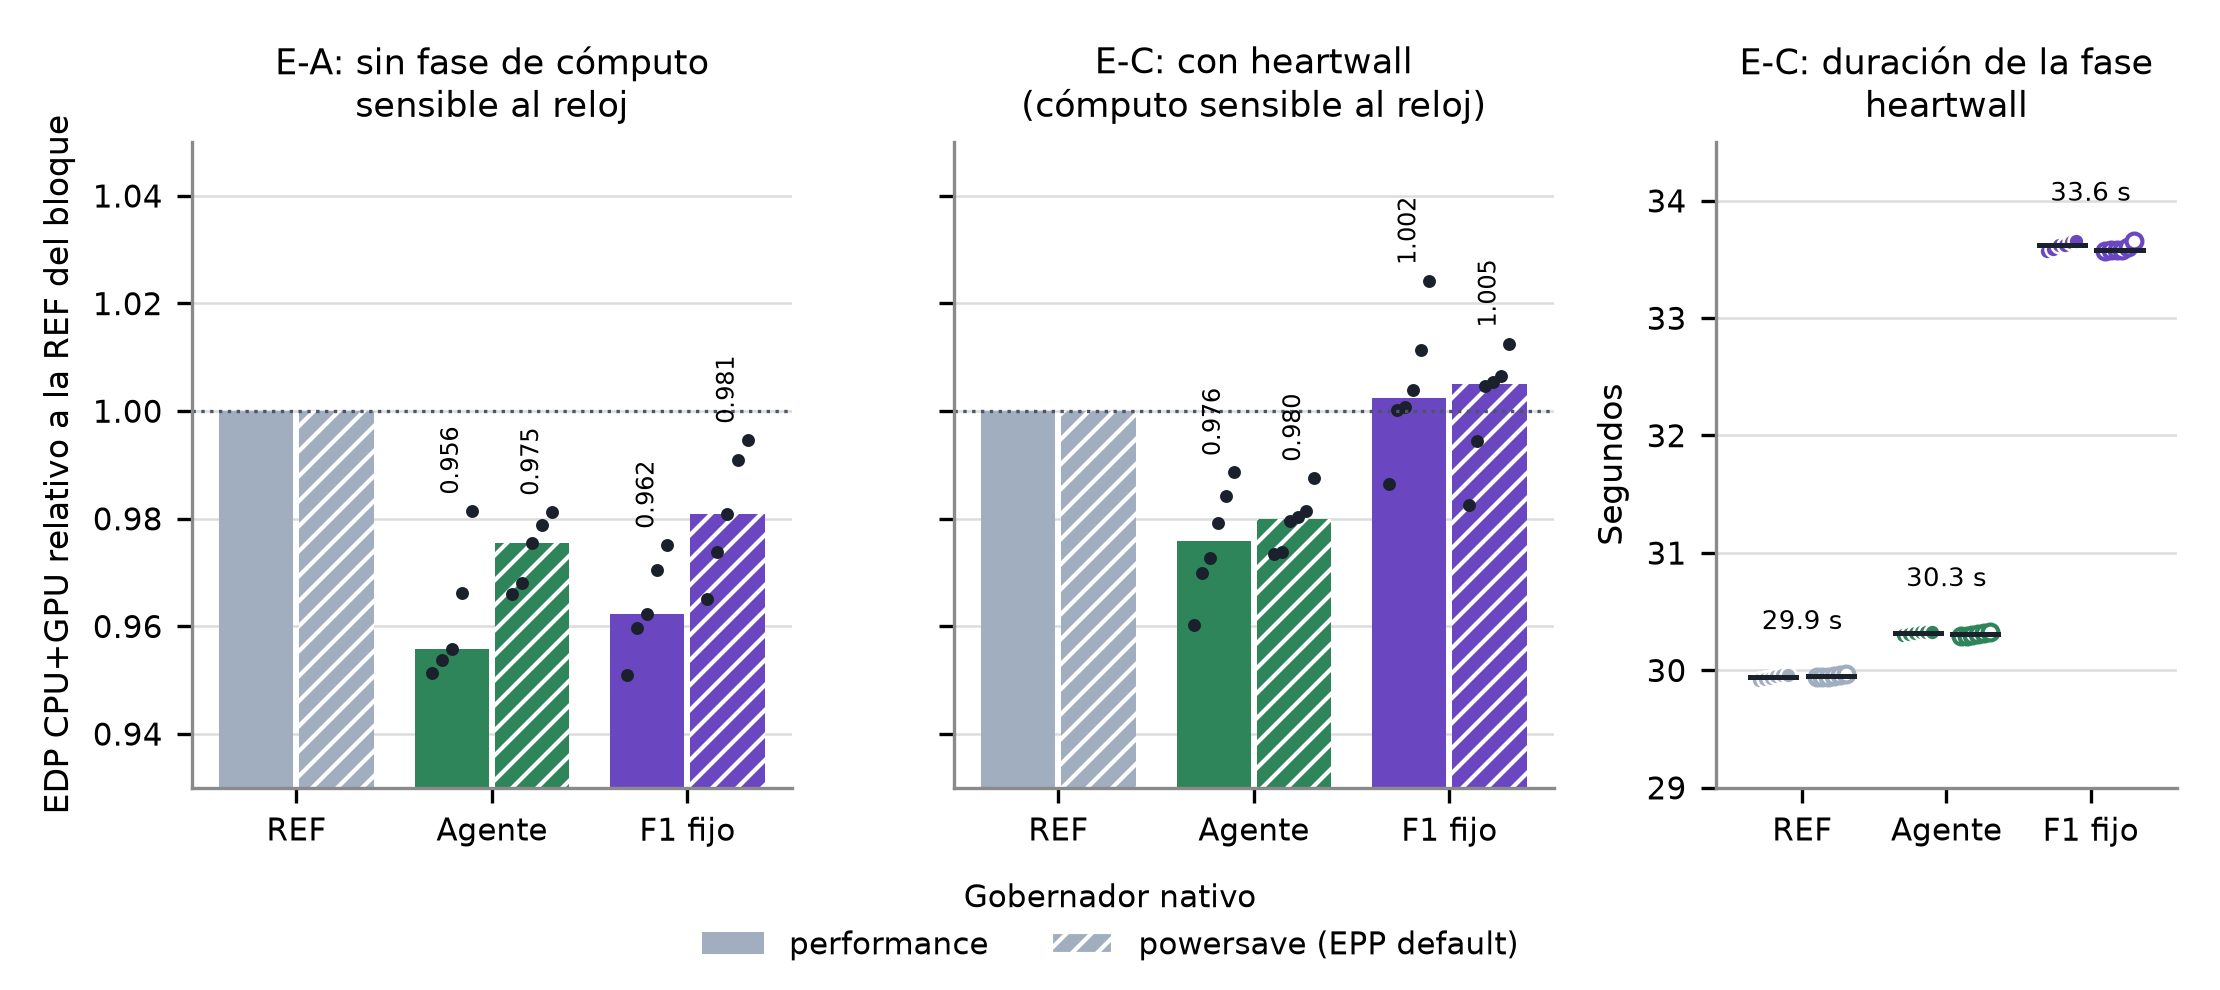
\includegraphics[width=0.66\textwidth]{fig_fase4_EC_20260930.png}

  \vspace{1mm}
  \begin{minipage}[t]{0.32\textwidth}
    \begin{card}[height=13mm,valign=center,fontupper=\tiny]
      \textbf{E-A:} agente/F1 fijo = 0.998 (IC95 0.990--1.006). DGEMM ya corría bajo 1260 MHz
      por el límite de potencia
    \end{card}
  \end{minipage}\hfill
  \begin{minipage}[t]{0.32\textwidth}
    \begin{cardhi}[height=13mm,valign=center,fontupper=\tiny]
      \textbf{E-C:} agente/F1 fijo = \textbf{0.972} (IC95 0.958--0.985); 6 de 6 bloques,
      $p=0.031$. Frente a la base: 0.976 ($p=0.031$)
    \end{cardhi}
  \end{minipage}\hfill
  \begin{minipage}[t]{0.32\textwidth}
    \begin{card}[height=13mm,valign=center,fontupper=\tiny]
      \textbf{heartwall:} 29.9 s base · 30.3 s agente · 33.6 s F1 fijo.
      F1 fijo no mejora la base (1.004)
    \end{card}
  \end{minipage}
  \notapie{E-C es una prueba de mecanismo: escenario construido con el kernel más favorable y una familia vista. En E-B (exploratorio), cuando el agente se abstuvo, F1 fijo ahorró más.}
\end{frame}

\subseccion{¿Qué no funcionó?}
\newcommand{\nocard}[2]{%
  \begin{card}[height=19mm,valign=center]
    \begin{tabular}{@{}m{8mm}@{}m{0.8\linewidth}@{}}
      \nomark & {\footnotesize\bfseries #1}\par\vspace{0.6mm}{\scriptsize #2}
    \end{tabular}
  \end{card}}
\begin{frame}{El agente no ganó en CPU, en LAMMPS ni en familias GPU no vistas}
  \vspace{4mm}
  \begin{columns}[T]
    \begin{column}{0.48\textwidth}
      \nocard{CPU}{Piso de potencia del 84 \%: la política es no actuar y el proceso de observación aumenta el EDP}
      \nocard{Familias GPU inéditas}{BabelStream: abstención en 9 de 11 repeticiones (E-B); quedó cerca de la paridad}
    \end{column}
    \begin{column}{0.48\textwidth}
      \nocard{LAMMPS}{EDP entre 1.003 y 1.009 de la base; el agente nunca aplicó F1}
      \nocard{Alcance}{Un solo nodo; modelo GPU entrenado por corrida y aplicado en ventanas de 3~s}
    \end{column}
  \end{columns}
\end{frame}
